\documentclass{article}[18pt]
\usepackage{../../../../format}
\lhead{CSys}
\usepackage{minted}

\begin{document}
\begin{center}
\underline{\huge Databases}
\end{center}
\textbf{Relation} - A table (with rows and columns)\\
\textbf{Attribute}  - A named column of a relation\\
\textbf{Domain} - The set of allowable values for an attribute\\
\textbf{Tuple} - A row of a relation\\
\textbf{Cell} - The intersection of a row and column\\
\textbf{Degree} - The number of attributes of a relation\\
\textbf{Cardinality} - The number of tuples of a relation
\section{Keys}
\textbf{Candidate Key} - A minimal (not minimum) set of attributes whose values uniquely identify the tuples\\
\textbf{Primary Key} - The candidate key selected to identify rows uniquely within the table\\
\textbf{Alternate Key} - Those candidate key(s) not selected as a primary key\\
\textbf{Simple Key} - The key consists of only one attribute\\
\textbf{Composite Key} - The key consists of only one several attributes\\
\textbf{Foreign Key} - An attribute in a table whose values must:
\begin{itemize}
	\item Either match the primary key in another table
	\item Be NULL
\end{itemize}
\section{Integrity Constraints}
\textbf{Entity integrity} - Every attribute of a primary key can not be null\\
\\
Purpose of entity integrity:
\begin{itemize}
	\item Guarantees each entity has a unique identifier
	\item Ensures that foreign key values can reference primary key values
\end{itemize}
\textbf{Referential integrity}
\begin{itemize}
	\item A foreign key either matches the primary key in the table it refers to
	\item or it is null
\end{itemize}
Referential integrity exists so that a reference between tables is value and prevents deleting a primary key that mas a matching foreign key
\section{Entity Relation Model}
Objective of the ER model:
\begin{itemize}
	\item Helps understanding of the nature and relationships among the data
	\item Helps derive tables in the Relational Data Model
\end{itemize}
Basic concepts:
\begin{itemize}
	\item Important data objects (entities)
	\item Important properties of the entities (attributes)
	\item Associations between entities (relationships)
\end{itemize}
There is also the constraints of entities, relationships and attributes
\subsection{Main concepts}
Entity
\begin{itemize}
	\item Any real thing that we recognise as a separate concern within the database
	\item Represented by rectangles
	\begin{center}
		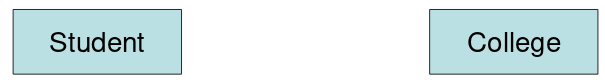
\includegraphics[scale=0.7]{Entity}
	\end{center}
\end{itemize}
Relationship
\begin{itemize}
	\item A names association between two entity types
	\item Represented by a labelled line connecting two entities
	\begin{center}
		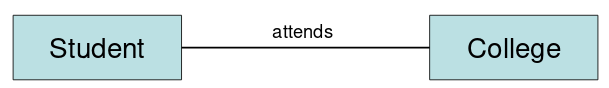
\includegraphics[scale=0.7]{Relationship}
	\end{center}
\end{itemize}
\section{Cardinality}
\textbf{Cardinality} - The number of entity occurrences that are related to a single occurrence of an associated entity type through this relationship
\begin{center}
	\includegraphics[scale=0.7]{"Crow's Foot"}
\end{center}
\section{Optionality and Participation}
If a teacher is employed by one or zero schools, it is denoted like so:
\begin{center}
	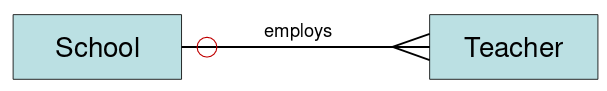
\includegraphics[scale=0.7]{Optionality}
\end{center}
If an entity participates optionality in a relationship:
\begin{itemize}
	\item It has partial participation
	\item Otherwise it has total participation
\end{itemize}
To say one school employs at least one Teacher, you would do it like so
\begin{center}
	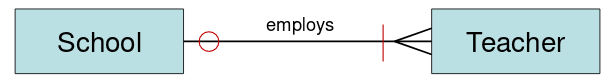
\includegraphics[scale=0.7]{Participation}
\end{center}
\section{Many to many relationships}
Many to many relationships are not allowed in the ER model, so we introduce a new entity, for example if you have the relationship
\begin{center}
	\includegraphics[scale=0.7]{"Many to Many"}
\end{center}
Introducing a new entity will resolve this
\begin{center}
	\includegraphics[scale=0.7]{"Many to Many1"}
\end{center}
\section{Functional data dependencies}
\textbf{Functional data dependency} - Describes the relationship among attributes in the same relation\\
For example "B is functionally dependent on A" if each value of A is associated with exactly one value of B\\
Informally if we know the attribute values of the set A then we know the unique values for the set B\\
\\
In a functional data dependency ($A\rightarrow B$)
\begin{itemize}
	\item Determinant - The set of all attributes on the left hand side (A)
	\item Dependent - The set of all attributes on the right hand side (B)
\end{itemize}
\textbf{Full functional dependency} - B is functionally dependent on A and B is not functionally dependent on any proper subset of A\\
\textbf{Partial functional dependency} - B is functionally dependent on A and B remains functionally dependent on at least one proper subset of A\\
\textbf{Transitive functional dependency} - If there exists functional dependencies $A\rightarrow B$ and $B\rightarrow C$ then the functional dependency $A\rightarrow C$ also exists
\section{First Normal Form}
A table is in First normal form if it has:
\begin{itemize}
	\item No repeating groups (every cell has one value)
	\item No identical rows
\end{itemize}
\section{Second Normal Form}
A table is in Second Normal Form if:
\begin{itemize}
	\item It is in 1NF and
	\item There is no partial functional dependencies - every non-key attribute is dependent on the whole primary key
\end{itemize}
When the primary key has only one attribute, if the table is in 1NF, it is also in 2NF\\
To bring a table into 2NF:
\begin{itemize}
	\item Remove any partially dependent attributes
	\item Place them in a new relation, along with the copy of their determinant
\end{itemize}
This is not in 2NF:
\begin{center}
	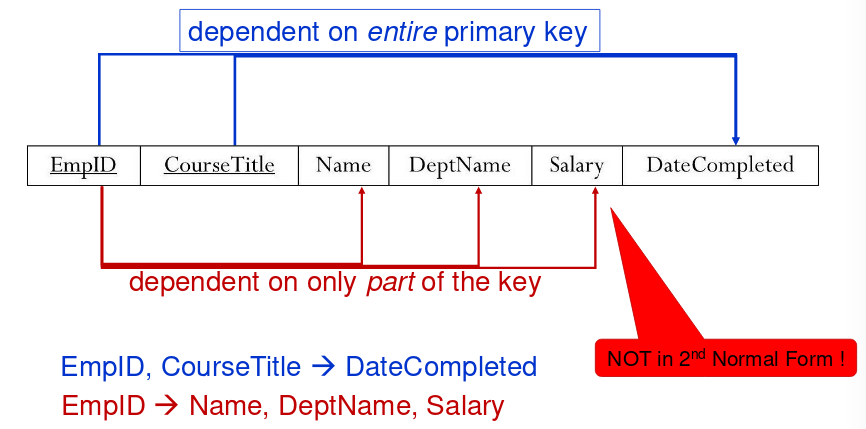
\includegraphics[scale=0.7]{2NF}
\end{center}
Example (converted in 2NF) has it decomposed into two separate relations
\begin{center}
	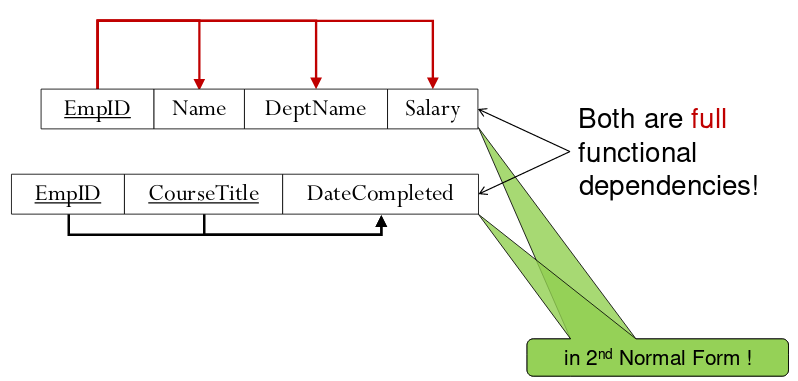
\includegraphics[scale=0.7]{2NF1}
\end{center}
\section{Third Normal Form}
A table is in Third Normal Form if:
\begin{itemize}
	\item It is in 2NF
	\item There are no transitive functional dependencies e.e. no non-key attribute is transitively dependent on the primary key
\end{itemize}
In other words, in 3NF all attributes (which are not part of the primary key) are functionally dependent on the key, the whole key, and nothing but the key\\
\\
How to bring a table into 3NF:
\begin{itemize}
	\item Remove the transitively dependent attributes
	\item Place them in a new relation
	\item Take the attributes of their determinant as the primary key in the new table
\end{itemize}
\section{SQL Queries}
An example of nested queries
\begin{minted}{sql}
SELECT staffNo, fName, IName, position
FROM Staff
WHERE branchNo=
	(SELECT branchNo
	FROM Branch
	WHERE street='163 Main St')
\end{minted}
\end{document}